\section{Fingertip detection}
In order to draw points using finger information, we have to detect the location of the fingertip.
If the gesture is 'draw (one finger)', we detect the fingertip of the index finger. 
If the gesture is 'erase (three fingers)' or 'move (two fingers)', we detect the fingertip of the middle finger. \par
We assume the fingertip is the further point from the center of the mass and also not the wrist side.
Our environment allows us to assume the wrist side is always top of the image, we simply find the furthest point from the center of the mass among the bottom half of the mask.

This function is implemented in fingertip.py. 

Fig. \ref{fig:finger} shows the results of the finger tip detection.
This method detects the finger tip correctly when the gesture is one finger or two fingers.
When the gesture is three fingers, the method sometimes detect the location between middle finger and other fingers.
Table \ref{tb:finger} shows the result of detected finger tip when the gesture is 'three fingers'.
We tried 143 frames of three fingers.
The error ratio is 12 \%. Fig. \ref{fig:errorfinger} shows the examples of failure. As we can see, it fails when the hand is not on the canvas. This would cause about 10 pixels error in video image and cause about 20 pixels error in canvas. This is about 3\% of the average length of the canvas.

\begin{figure}[htbp]
 \centering
 \begin{tabular}{lllll}
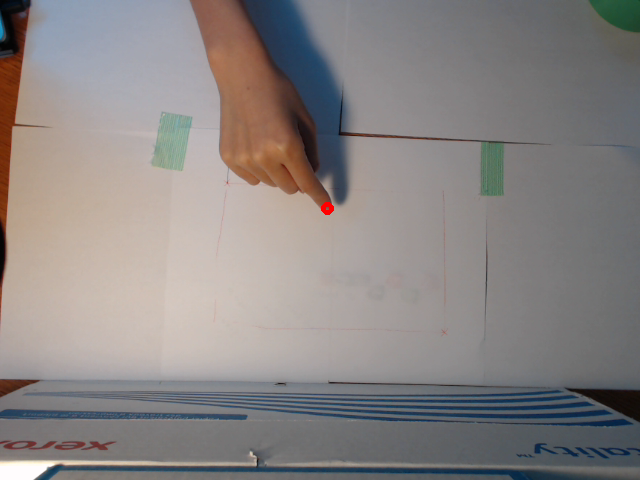
\includegraphics[width=5cm]{fig3/im1_13.png} &
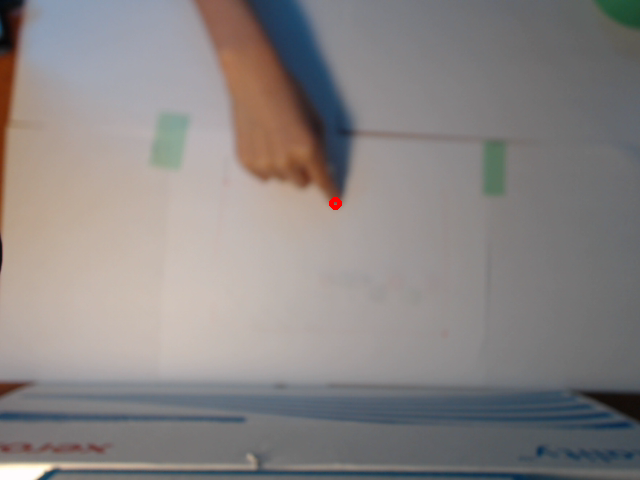
\includegraphics[width=5cm]{fig3/im1_55.png} \\
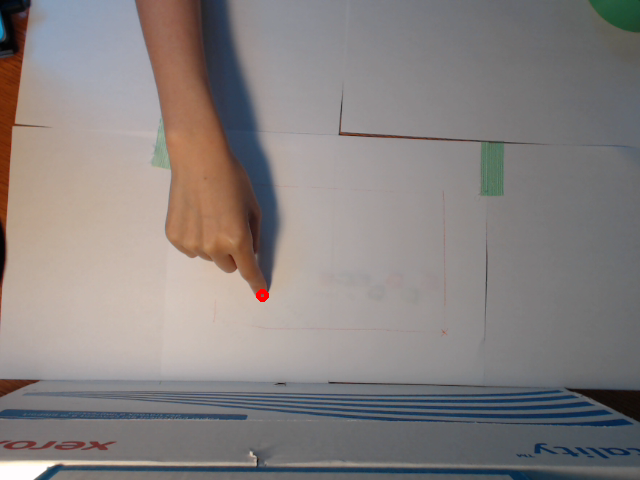
\includegraphics[width=5cm]{fig3/im1_67.png} &
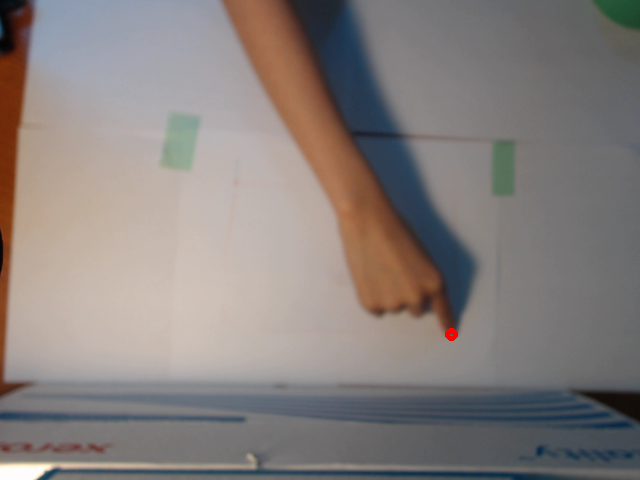
\includegraphics[width=5cm]{fig3/im1_146.png} \\
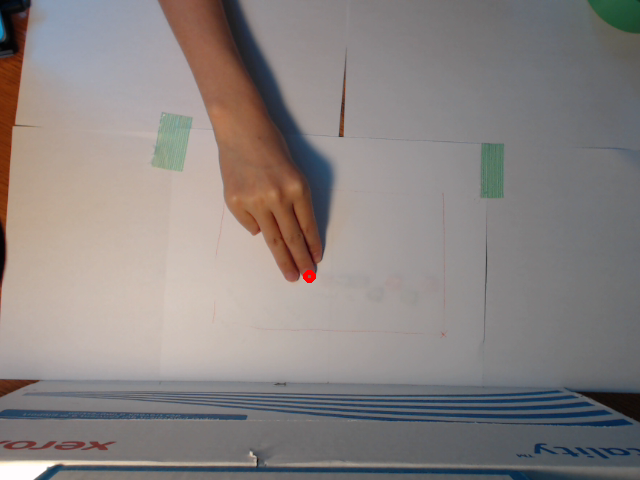
\includegraphics[width=5cm]{fig3/im2_26.png} &
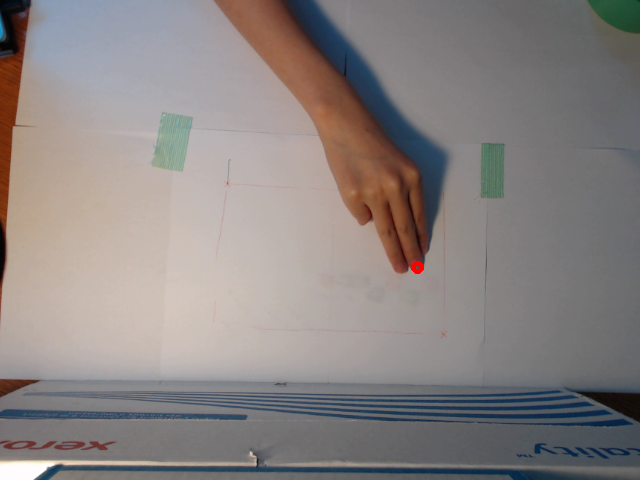
\includegraphics[width=5cm]{fig3/im2_98.png} \\
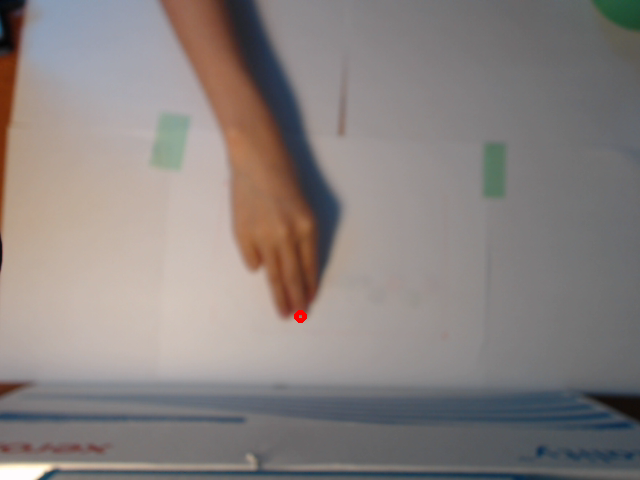
\includegraphics[width=5cm]{fig3/im2_149.png} &
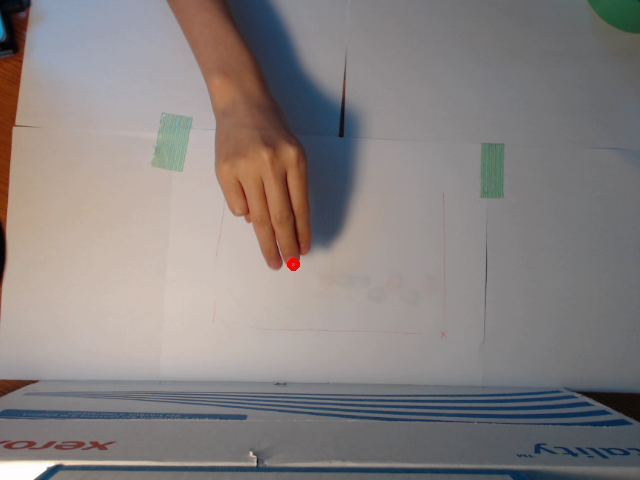
\includegraphics[width=5cm]{fig3/im2_162.png} \\
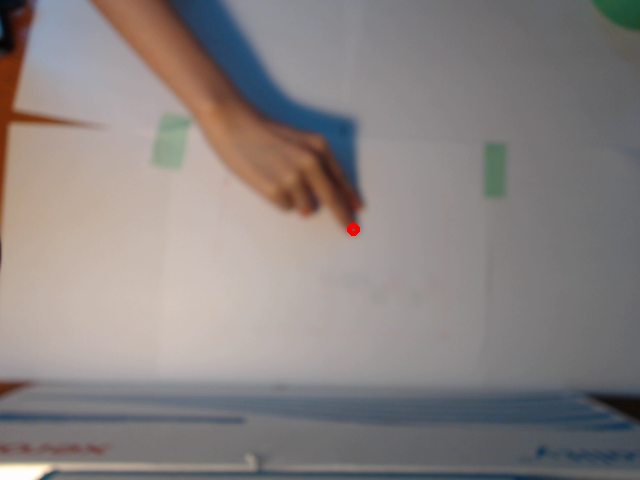
\includegraphics[width=5cm]{fig3/im3_78.png} &
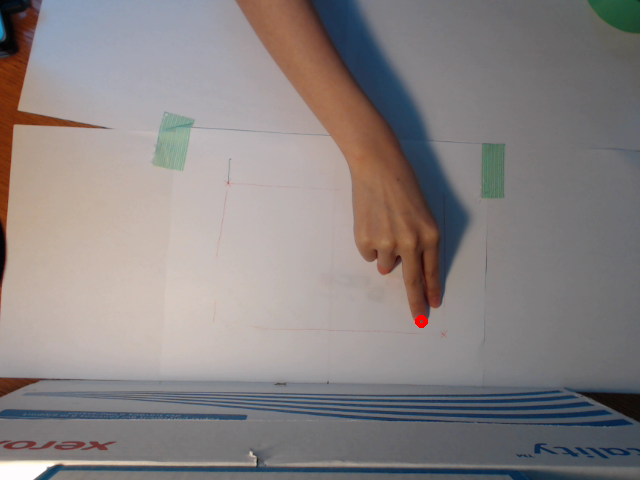
\includegraphics[width=5cm]{fig3/im3_109.png} \\
\end{tabular}

 \caption{The results of finger detection}
\label{fig:finger}
\end{figure}

\begin{figure}[htbp]
 \centering
 \begin{tabular}{lll}
	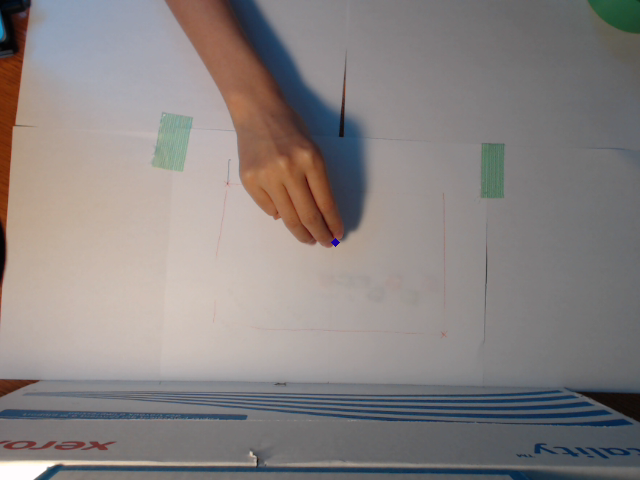
\includegraphics[width=5cm]{fig2/im2_109.png} &
	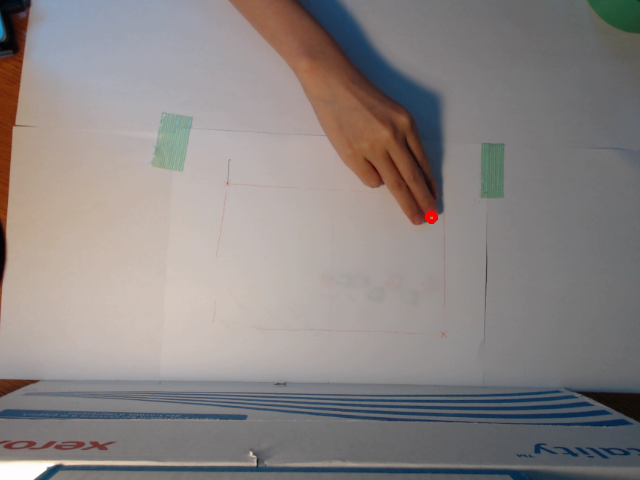
\includegraphics[width=5cm]{fig2/im2_133.png} \\
  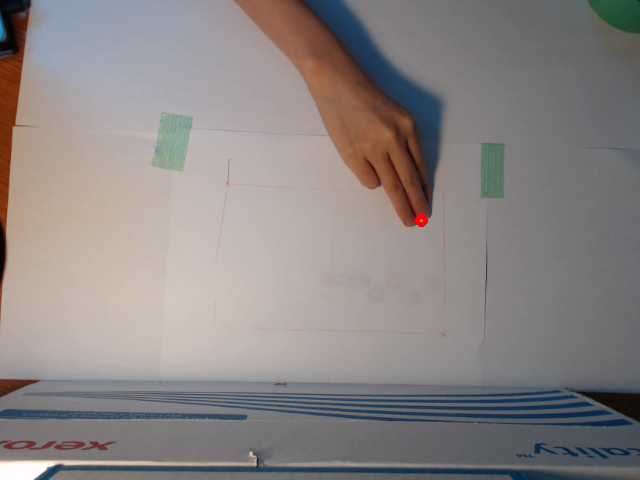
\includegraphics[width=5cm]{fig2/im2_138.png}&
	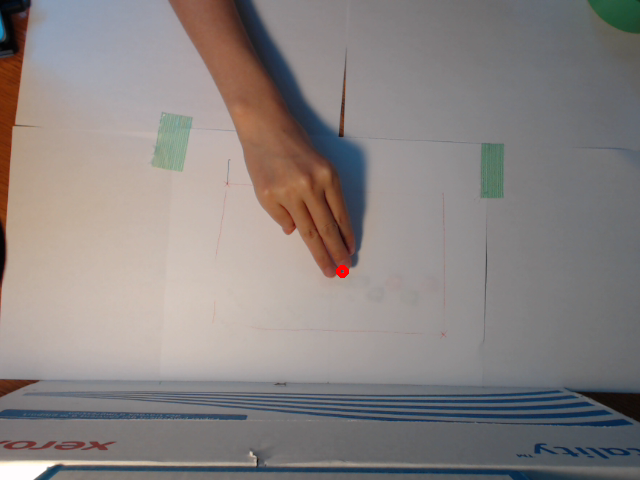
\includegraphics[width=5cm]{fig2/im2_4.png}  \\
	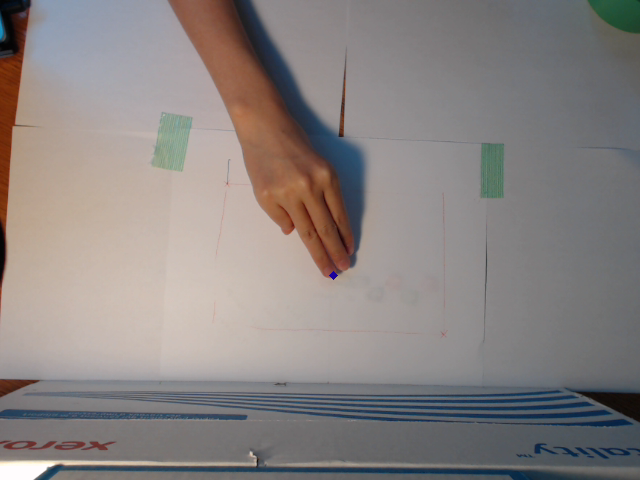
\includegraphics[width=5cm]{fig2/im2_5.png}  &
	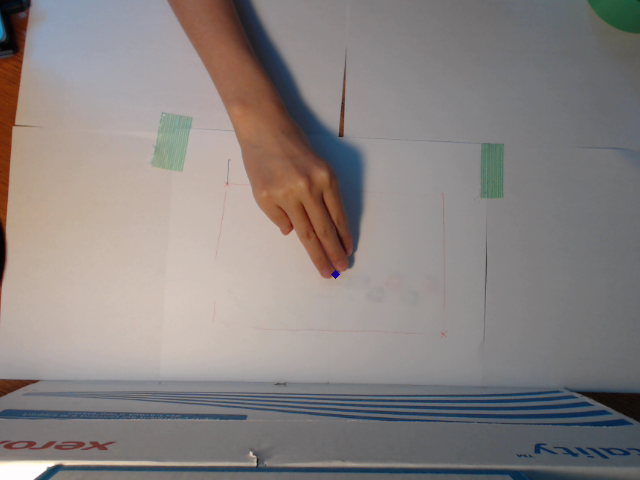
\includegraphics[width=5cm]{fig2/im2_6.png}
\end{tabular}

 \caption{The errors}
\label{fig:errorfinger}
\end{figure}

\begin{table}
 \caption{The result of three fingers' finger tip detection}
 \label{tb:finger}
 \begin{tabular}{|c|c|}
 \hline
 The location of the result &  \\ \hline
 Index finger & 0(0\%) \\ \hline
 Between index finger and middle finger & 1(0\%) \\ \hline
 Middle finger & 124 (87\%) \\ \hline
 Between middle finger and third finger & 12(8\%) \\ \hline
 Third finger & 6(4\%) \\ \hline
 Total & 143 \\ \hline
 \end{tabular}
\end{table}
